% !TEX root = UAV_Landing_Pad.tex

\chapter{Overview and concept of operations}
%Note Link this shit.
Commensurate with the User Stories and Architecute Design, we have isolated three key components.  These are intrinsic to performing the operations of UAV, UGV, and common ROS-based infrastructure.  To better illustrate these components, this section will overview the operational entities as semi-independent sections.


\section{Scope}
This section of the Senior Design documentation covers the three main components that are being constructed to deliver upon the aforementioned User Stories.


\section{Purpose}
This system will assist in the collection of data in otherwise unsafe zones for human occupancy as it relates to:

  \begin{itemize}
    \item Natural Disaster Reconnaissance
    \item Forest Fires - Spread and Destructive Evaluation
    \item Missing Persons Tracking
  \end{itemize}


\subsection{UAV}
The Unmanned Arial Vehicle will fulfill the reconnaissance tasks in this project. This will consist of video and sensor data collection, while in flight.  Upon completion of data collection this data will be transfered back to a control base station via radio telemetry.  It is crucial that the UAV be able to return to the ground vehicle before energy reserves are depleted to recharge and be transported securly to the next location where data collection can begin again.\newline



The current configuration for this component is:
  \begin{itemize}
    \item AMP 2.6 - flight control board
    \item 3dr ublox GPS with Compass - compass and gps
    \item R5800X receiver and TXV582 - video transmitting
    \item Sony HAD 520 line camera - on board camera
    \item Spektrum AR7000 - 7 channel receiver
    \item 915 MHz radio - telemetry with ground station
  \end{itemize}

\subsection{UGV}
The Unmanned Ground vehicle is computationally more simplistic than the UAV and will fulfill the tasks of navigation to pre-determined GPS coordinates, elevate the launch pad, wait for return of the UAV and recharge the UAV on arrival.  The system is set to include the following components after the frame has been constructed in Sprinter Break:\newline

  \begin{itemize}

    \item[] The current ground vehicle loadout contains the following components:
    \item GPS – Make and model still under investigation
    \item SLAM Cameras (Asus Xtioc \& Microsoft Kinect)
    \item Recharging Station with mounts
    \item Tilting platform with LED indicators for low light environments.
    \item Power supply
    \item Odroid computational units.  Likely Odroid XU 3 models.

  \end{itemize}

\begin{figure}[tbh]
\begin{center}
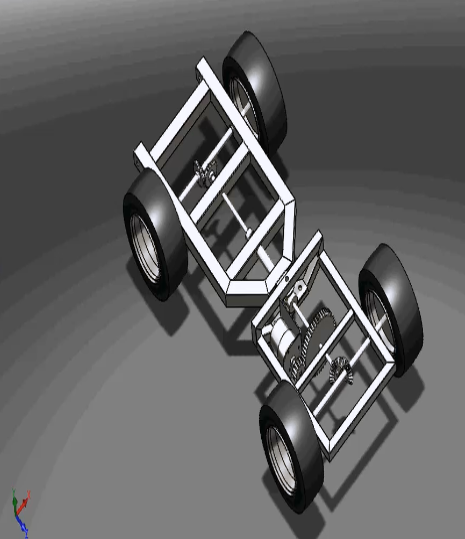
\includegraphics[width=0.50\textwidth]{resources/img/UGV}
\end{center}
\caption{Frame proposed for UGV \label{systemdiagram}}
\end{figure}

\subsection{Common Components}
To better distribute work load as well as reduce the testing required for new software developments in ROS, Eye in the Sky has proposed to create common infrastructure programming for input devices.  This common protocol will take various input streams (Cameras - Stereo and Monocular, GPS, Motor Control, etc.) and will use common topics or service subscriptions to streamline communication between these devices.  This will further assist with common computation such as GPS interpretation.

\section{Systems Goals}
This completed system is intended to:\newline

  \begin{enumerate}

    \item (UGV) Take predetermined GPS waypoint data and navigate to a location to begin reconnaissance.
    \item (UGV) Once at the location, level the landing platform to launch the UAV \& disconnect any charging and securing mechanisms.
    \item (UAV) Start mapping and elevate to a predetermined altitude directly above the UAV and navigate linearly to a perimiter of a flight circle.
    \item (UAV) Once on the radius of the flight path, begin traversing the path while recording video and other sensor data.
    \item (UAV) After completing the flight path, return to the UAV with both visual and mapping assistance.
    \item (UAV) Orient for landing and touch down on the UAV's platform.
    \item (UGV) Secure the UAV and begin charging.

  \end{enumerate}

This process is scheduled to repeat until the UGV has expired all GPS way-points.  At this time the UGV will return to the start location or any ending location for retrieval by the owners.

\section{System Overview and Diagram}
To illustrate the connectivity of these various components, the following system diagram has been created.

\begin{figure}[tbh]
\begin{center}
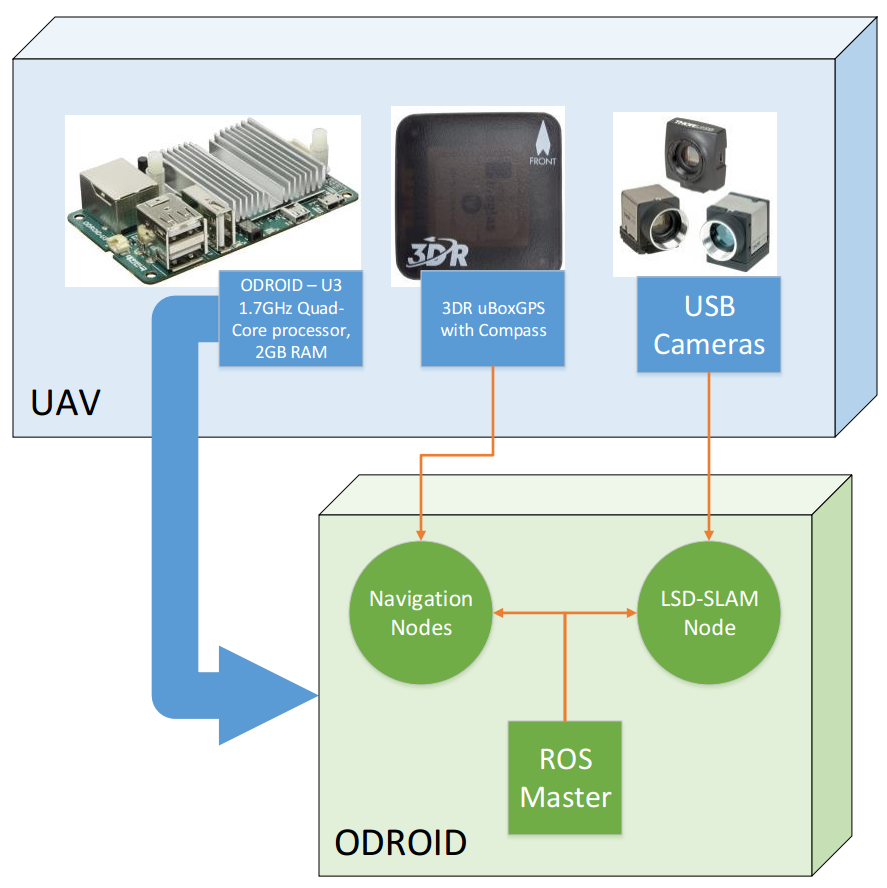
\includegraphics[width=0.5\textwidth]{resources/diagram/SysDiagUAV}
\end{center}
\caption{UAV System Diagram \label{systemdiagram}}
\end{figure}


\begin{figure}[tbh]
\begin{center}
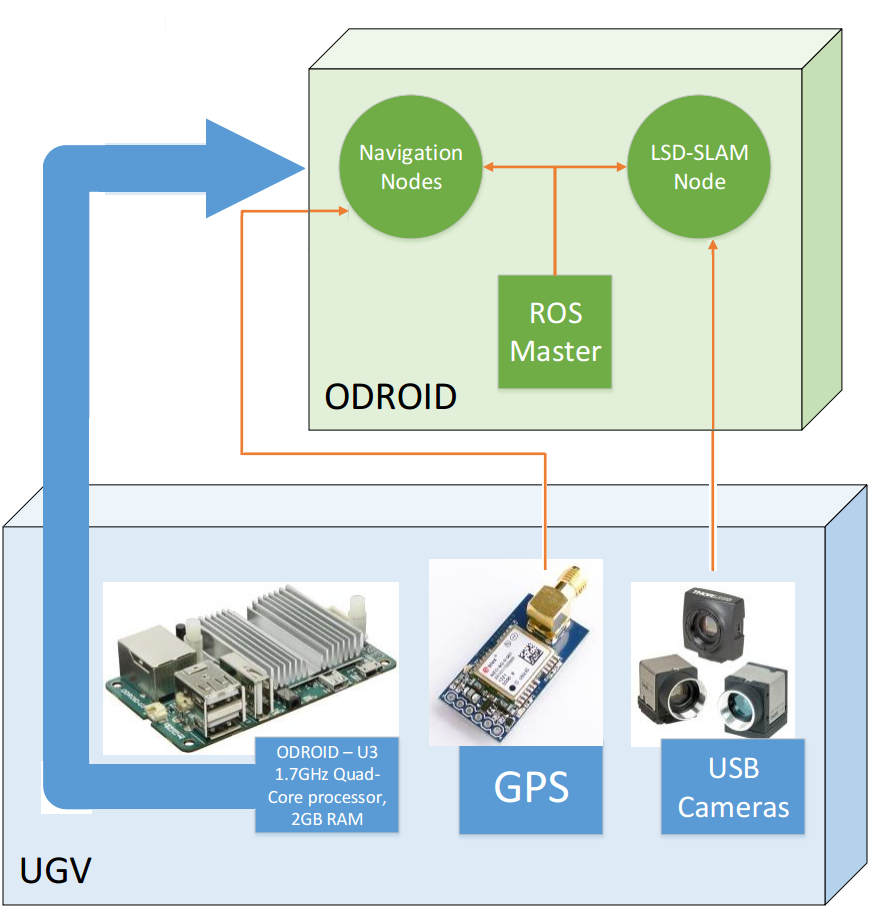
\includegraphics[width=0.5\textwidth]{resources/diagram/SysDiagUGV}
\end{center}
\caption{UGV System Diagram \label{systemdiagram}}
\end{figure}


\section{Technologies Overview}
A brief list of the technologies included and their applications:


  \begin{enumerate}

    \item OpenCV
      \begin{enumerate}

        \item Distance Detection to known design on Landing Pad
        \item Possible Homography integration

      \end{enumerate}
    \item SLAM
      \begin{enumerate}

        \item Varieties Used
          \begin{enumerate}

            \item Hector-SLAM - Integrated with UAV mapping structure
            \item LSD-SLAM - Additional mapping and localization for UAV
            \item Point Cloud Maps- Obsticle and path detection for UGV

          \end{enumerate}
      \end{enumerate}

    \item GPS - Global coordination and additional verification on UAV / UGV localization.

  \end{enumerate}
